%!TEX program = xelatex
\documentclass[fleqn]{beamer}
\usetheme{metropolis}
\usepackage{graphicx}
\usepackage{comment}
\usepackage{color}
\usepackage[super]{nth}
\title{Image segmentation using SCIP}
\subtitle{}
\date{\today}
\author{Robert Schütz, Daniela Kilian}
\institute{Advanced project SS 2017}

\usepackage{mathtools}

\newcommand{\superpixels}{\mathcal{S}}
\newcommand{\segments}{\mathcal{P}}

\begin{document}
	\maketitle
	
	\begin{frame}{Content}
		\setbeamertemplate{section in toc}[sections numbered]
		\tableofcontents
	\end{frame}

	\section{Problem description}
	\begin{frame}{Task}
		TODO
	\end{frame}	
	
	\begin{frame}{Master problem}
		\begin{figure}
			\centering
				%\input{data_image.pdf_tex}
				\caption{Input image}
			
		\end{figure}
	\end{frame}
	
	\begin{frame}{Master problem}
		\begin{figure}
			\centering
			%\input{data_superpixels.pdf_tex}
		\end{figure}
	\end{frame}
	
	\begin{frame}{Master problem}
		\begin{figure}
			\centering
			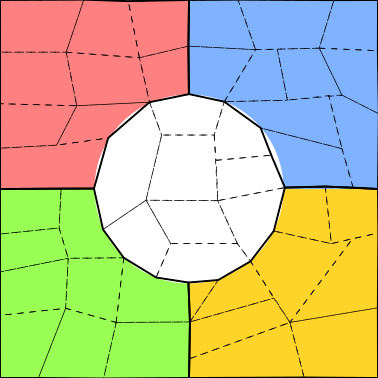
\includegraphics[scale=.5]{data_segments.png}
			\caption{Selected segments}
		\end{figure}
	\end{frame}

    \begin{frame}{Master problem}
        Given data in the theoretical formulation of the master problem:
        \begin{itemize}
            \item $\superpixels$: set of superpixels
            \item $\segments$: set of segments %sagen: connected
            \item $y_s\geq0$: color of superpixel $s\in\superpixels$
            \item $T\subseteq\superpixels$: set of master nodes %number of segments to select = #T
            \item $k=|T|$: number of segments to cover the image with
            \item $r_P=\sum_{s\in P}|y_t-y_s|$: error of segment $P\in\segments$,
            where $t\in T$ is the single master node for which $t\in P$
        \end{itemize}
    \end{frame}
	
	\begin{frame}{Master problem}
		There is a binary variable $x_P$ for every segment $P\in\segments$.
        
		The problem reads as follows:
		\begin{align}
    		&\min\quad \sum_{p\in\mathcal{P}} r_P\cdot x_P\\
		    &\text{s.t.}\quad \smashoperator{\sum_{\{P\in\mathcal{P}:s\in P\}}} x_P = 1 \quad\forall s\in\superpixels \\
		    &\phantom{\text{s.t.}\quad} \sum_{P\in\mathcal{P}} x_P = k \\
		    &\phantom{\text{s.t.}\quad} x_P \in \{0,1\}
		\end{align}
	\end{frame}
	
	\begin{frame}{Dual problem}
		The dual variables are
		\begin{itemize}
			\item $\mu_s, \forall s\in\superpixels$: corresponding to (2)
			\item $\lambda$: corresponding to (3)
		\end{itemize}
		
		The dual problem reads as follows:
		\begin{align}
		    &\max\quad \smashoperator{\sum_{s\in\superpixels}} \mu_s + k\cdot\lambda \\
		    &\text{s.t.}\quad \sum_{s\in P} \mu_s + \lambda \leq r_P \quad\forall P\in\mathcal{P} \\
		    &\phantom{\text{s.t.}\quad} \mu_s \text{ free} \\
		    &\phantom{\text{s.t.}\quad} \lambda \text{ free}
		\end{align}
	\end{frame}
	
	\begin{frame}{Pricing problem}
		There is a pricing problem for each master node $t\in T$,
		which generates a segment containing $t$.
		
		If $s\in\superpixels$ is in the new segment, then $x_s=1$.		
		 
		\begin{align}
    		&\min\quad -\sum_{s\in\superpixels} x_s\cdot\mu_s + \sum_{s\in\superpixels} x_s\cdot|y_t-y_s| \\
    		&\text{s.t.}\quad \text{connectivity constraints} \\
	    	&\phantom{\text{s.t.}\quad} x_s \in\{0,1\}
		\end{align}
	\end{frame}
	
	\begin{frame}{Pricing problem}
		Constraint (6) of the dual problem is violated by the new segment if and only if
		\[-\sum_{s\in\superpixels} x_s\cdot\mu_s + \underbrace{\sum_{s\in\superpixels} x_s\cdot|y_t-y_s|}_{=r_{\{s\in\superpixels\ :\ x_s=1\}}} < \lambda.\]
        
		Therefore, a new segment has to satisfy this inequality in order to be added to the master problem.
	\end{frame}
    
	\begin{frame}{Cutting planes}
		We use a cutting planes approach to ensure connectivity of the new segments.
        To this goal, we represent the superpixels as nodes in a graph.
        Two superpixels are connected if they have adjacent pixels in the original image.
		
		After solving the pricing problem,
		we look at the subgraph of all $s\in\superpixels$ for which $x_s=1$.
		If there is a component $C$ that is not connected to $t$,
		we add the following cut for each $s\in C$:
		\[\sum_{s'\in\delta(C)}x_{s'} \geq x_s\]
		
		%TODO ruby's bild
	\end{frame}
	
	\section{About SCIP}
	\begin{frame}{What is SCIP?}
		From \url{scip.zib.de}:
		\begin{quote}
			``SCIP is currently one of the fastest non-commercial solvers for mixed integer programming (MIP)
			and mixed integer nonlinear programming (MINLP).
			It is also a framework for constraint integer programming and branch-cut-and-price.''
		\end{quote}
	\end{frame}

    \begin{frame}{What is SCIP?}
        \begin{figure}
            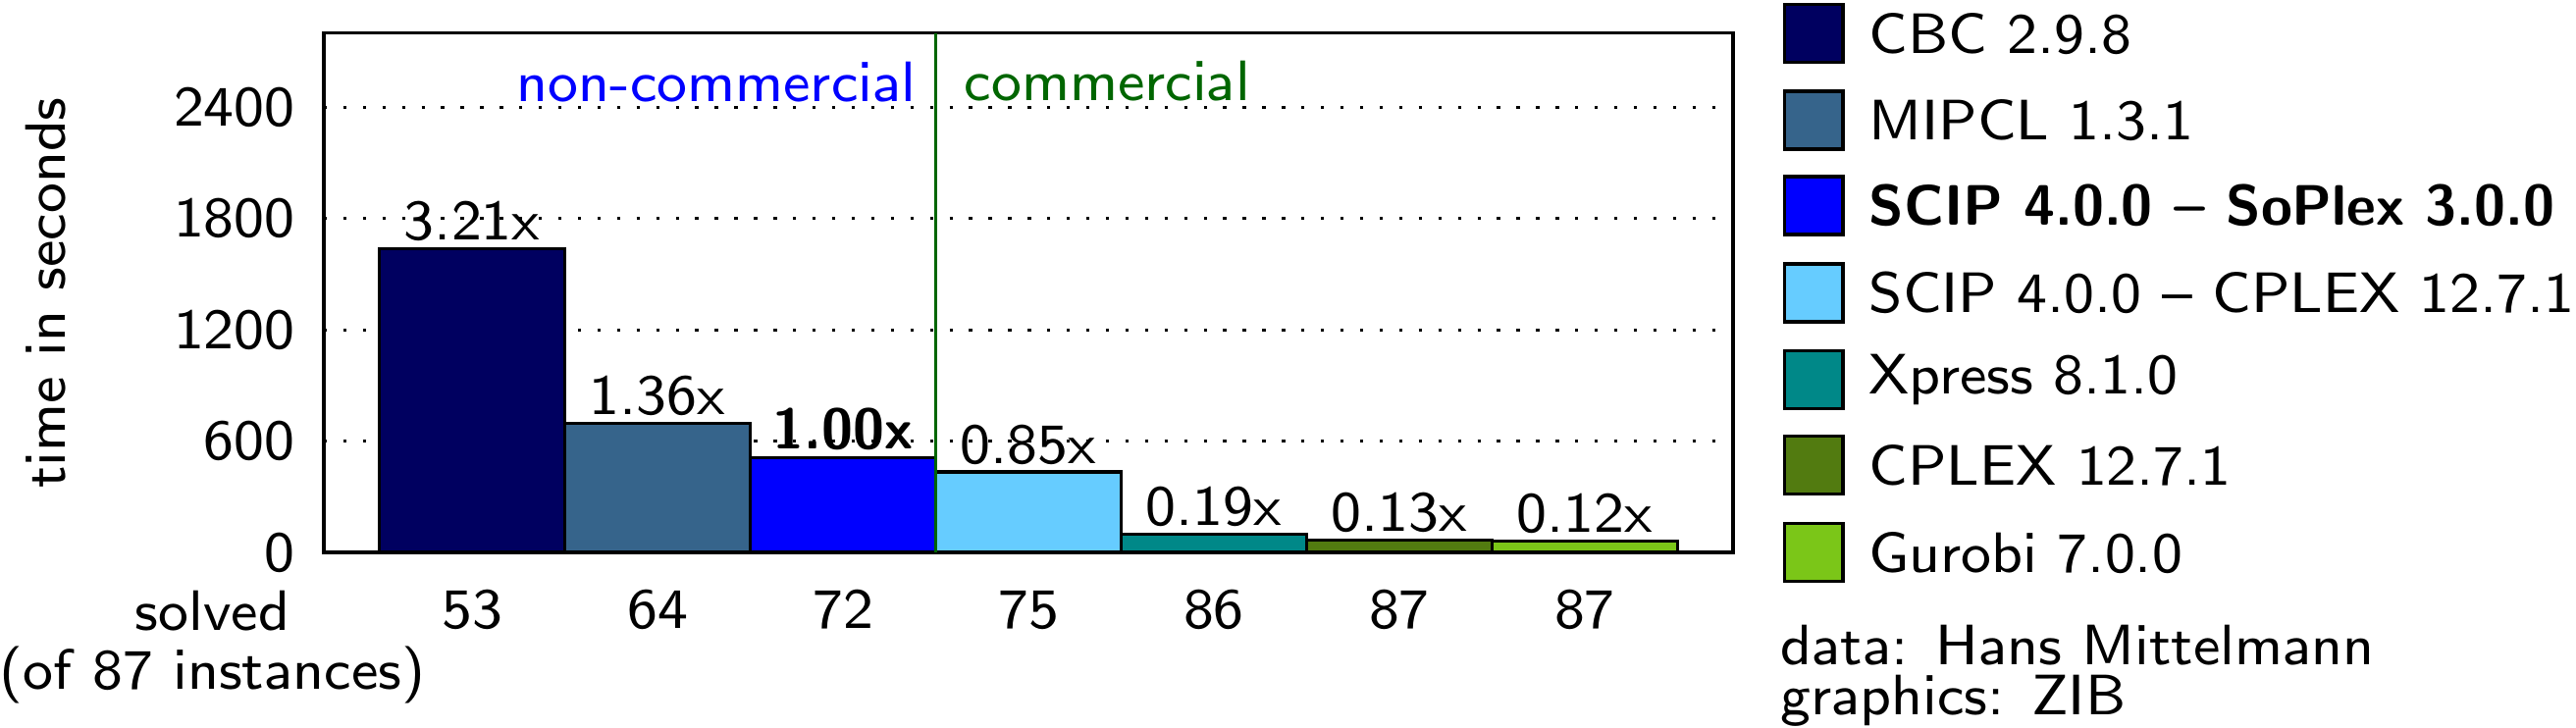
\includegraphics{comparison}
            \caption{MIP solver benchmark}
        \end{figure}
    \end{frame}

    \begin{frame}{What is SCIP?}
        SCIP is developed at the Zuse Institute Berlin.
        It is written in C, but can also be interfaced using
        \begin{itemize}
            \item C++
            \item Python
            \item Java
            \item \dots
        \end{itemize}
    
        SCIP can use different LP solvers, e.g.
        \begin{itemize}
            \item SoPlex % also developed at ZIB
            \item CPLEX
        \end{itemize}
    \end{frame}

    \begin{frame}{Advantages}
        Among others, SCIP has support for customizing the following aspects of the solution process:
        \begin{itemize}
            \item Constraint handlers % d.h. eigene Arten von constraints und auch cutting planes
            \item Separators
            \item Variable pricers
            \item Branching rules
        \end{itemize}
        Because these use callbacks, you do not have to write your own control loop.
        
        Also, SCIP can automatically do branching.
        You only need to specify that a certain variable should be binary/integral.
    \end{frame}
	
	\section{Implementation details}
    \begin{frame}{Programming Language}
        We're using C++.
        This makes it easy to interface with SCIP and add custom plugins.
        
        There are multiple SCIP examples written in C++, notably
        \begin{itemize}
            \item \textbf{VRP}, involving a custom pricer % vehicle routing problem
            \item \textbf{TSP}, involving a custom constraint handler % travelling salesman problem
        \end{itemize}
        We started off of these and implemented the desired functionality.
    \end{frame}
    
	\section{Possible improvements}
    \begin{frame}{Pricing heuristic}
        
    \end{frame}

    \begin{frame}{Branching rules}
        content...
    \end{frame}
    
    \section{Demo}
\end{document} 
